\chapter{Funciones de onda, matrices de densidad y localidad}

\lectureoverview{El teorema de Bell se pospone por una razón esencial: antes de preguntar qué prohíbe Bell, debemos decir con precisión qué es el entrelazamiento. Un estado bipartito está entrelazado cuando no puede factorizarse en un estado para Alice y otro para Bob. Las funciones de onda hacen concreto este criterio, las correlaciones revelan sus consecuencias y el singlete ofrece el ejemplo decisivo. La matriz de densidad reducida se convierte entonces en la descripción local completa de una parte de un todo entrelazado. Con estas herramientas, la medición aparece como una interacción que entrelaza; la frontera sistema--observador puede desplazarse sin cambiar las predicciones, y la aparente tensión entre entrelazamiento y localidad puede formularse con precisión: las elecciones distantes cambian las correlaciones condicionadas, pero no las estadísticas no condicionadas disponibles para transmitir señales.}

\section{Qué significa realmente el entrelazamiento}

Resulta tentador pasar directamente al teorema de Bell. El teorema es hermoso, pero su importancia no puede separarse de la estructura que pone a prueba. Por eso, la pregunta más urgente aún no es si la mecánica cuántica viola una desigualdad de Bell, sino qué dice un estado entrelazado sobre un sistema compuesto.

Una expresión habitual es que dos sistemas entrelazados \emph{comparten un estado}. Esa expresión no distingue nada. Todo sistema compuesto tiene un estado, esté o no entrelazado. La distinción está en la factorización. Si \(A\) y \(B\) tienen espacios de Hilbert \(\mathcal H_A\) y \(\mathcal H_B\), el estado del par pertenece a
\begin{equation}
\mathcal H_{AB}=\mathcal H_A\otimes\mathcal H_B.
\end{equation}
Un estado puro es un estado producto si puede escribirse como
\begin{equation}
\ket{\Psi}_{AB}=\ket{\psi}_A\otimes\ket{\phi}_B.
\label{eq:l7-product-state}
\end{equation}
Si no existe tal par de factores, \(\ket{\Psi}_{AB}\) está entrelazado.

\begin{classroomqa}
\audiencequestion{¿El entrelazamiento significa simplemente que ambos sistemas aparecen en un mismo vector de estado?}
\lecturerresponse{No. Un estado producto también pertenece al espacio de Hilbert del par completo. El entrelazamiento es la afirmación más fuerte, independiente de la base, de que el vector del todo no puede escribirse como un vector para Alice multiplicado por otro para Bob.}
\end{classroomqa}

\begin{classroomqa}
\audiencequestion{¿Podría un cambio de base ingenioso convertir un estado entrelazado en uno producto?}
\lecturerresponse{No, si el cambio de base es local, es decir, si consiste en un cambio de base para Alice y otro para Bob. Los cambios de base locales alteran las coordenadas de cada factor, pero no modifican si el estado se factoriza. Una base completamente arbitraria del espacio de Hilbert conjunto puede ocultar la estructura de producto tensorial, pero no cambia qué grados de libertad físicos pertenecen a Alice y cuáles a Bob.}
\end{classroomqa}

\section{Las funciones de onda como coordenadas en el espacio de Hilbert}

La expresión \emph{función de onda} evoca imágenes históricas que no forman parte de su definición matemática. Una función de onda es la representación en coordenadas de un vector de estado en una base elegida. Sea un conjunto completo de observables que conmutan y cuyos autovectores simultáneos son
\begin{equation}
\ket{a,b,c,\ldots}.
\end{equation}
Las etiquetas deben ser completas: en conjunto, deben distinguir todos los vectores de la base. Entonces
\begin{align}
\ket{\Psi}
&=\sum_{a,b,c,\ldots}
\ket{a,b,c,\ldots}
\braket{a,b,c,\ldots}{\Psi} \\
&=\sum_{a,b,c,\ldots}
\psi(a,b,c,\ldots)\ket{a,b,c,\ldots},
\label{eq:l7-wavefunction-expansion}
\end{align}
donde
\begin{equation}
\psi(a,b,c,\ldots)
=\braket{a,b,c,\ldots}{\Psi}.
\label{eq:l7-wavefunction-definition}
\end{equation}
Para etiquetas continuas, las sumas correspondientes se convierten en integrales.

\begin{figure}[htbp]
\centering
\includegraphics[width=0.88\textwidth]{lecture_07_figure_01.png}
\caption{La función de onda como el conjunto de coeficientes de un estado en una base completa.}
\lectureframe{00:07:00}
\end{figure}

Para una partícula en el espacio tridimensional, las etiquetas que conmutan pueden ser \(x,y,z\), y
\begin{equation}
\psi(x,y,z)=\braket{x,y,z}{\Psi}
\end{equation}es la conocida función de onda de Schr\"odinger en el espacio de posiciones. Para un espín en la base \(\sigma_z\), la función de onda no es más que el par
\begin{equation}
\psi(u)=\braket{u}{\Psi},
\qquad
\psi(d)=\braket{d}{\Psi}.
\end{equation}
Para dos espines se necesitan dos etiquetas:
\begin{equation}
\Psi(a,b)=\braket{a,b}{\Psi},
\qquad
a,b\in\{u,d\}.
\label{eq:l7-two-spin-wavefunction}
\end{equation}
Esta definición no exige que haya una onda literal en el espacio.

\begin{classroomqa}
\audiencequestion{¿Cambiar la base de la función de onda equivale a una transformada de Fourier?}
\lecturerresponse{La transformada de Fourier es el cambio de base específico entre las representaciones de posición y de momento. En general, todo cambio de base ortonormal es una transformación unitaria de las coordenadas. Pasar de la base \(\sigma_z\) a la base \(\sigma_x\) es análogo a una transformada de Fourier, aunque se trata de una matriz unitaria de dimensión finita y no de una transformada integral de posición--momento.}
\end{classroomqa}

\begin{classroomqa}
\audiencequestion{Si la función de onda cambia al cambiar de base, ¿ha cambiado el estado físico?}
\lecturerresponse{No. El ket \(\ket{\Psi}\) es el estado abstracto. Los números \(\psi(a,b,c,\ldots)\) son sus coordenadas en una base seleccionada. Cambiar las coordenadas modifica esos números, pero deja intactos el vector y todas las predicciones físicas.}
\end{classroomqa}

\section{Valores esperados en componentes}

Antes de introducir las matrices de densidad, hagamos explícita la estructura en componentes de un valor esperado. Sea \(L\) un observable, con elementos de matriz
\begin{equation}
L_{a'a}=\bra{a'}L\ket{a}.
\label{eq:l7-matrix-elements}
\end{equation}
Si \(\ket{\Psi}=\sum_a\psi(a)\ket{a}\), entonces
\begin{align}
\expect{L}
&=\bra{\Psi}L\ket{\Psi} \\
&=\sum_{a',a}
\psi^*(a')\bra{a'}L\ket{a}\psi(a) \\
&=\sum_{a',a}\psi^*(a')L_{a'a}\psi(a).
\label{eq:l7-expectation-components}
\end{align}

\begin{figure}[htbp]
\centering
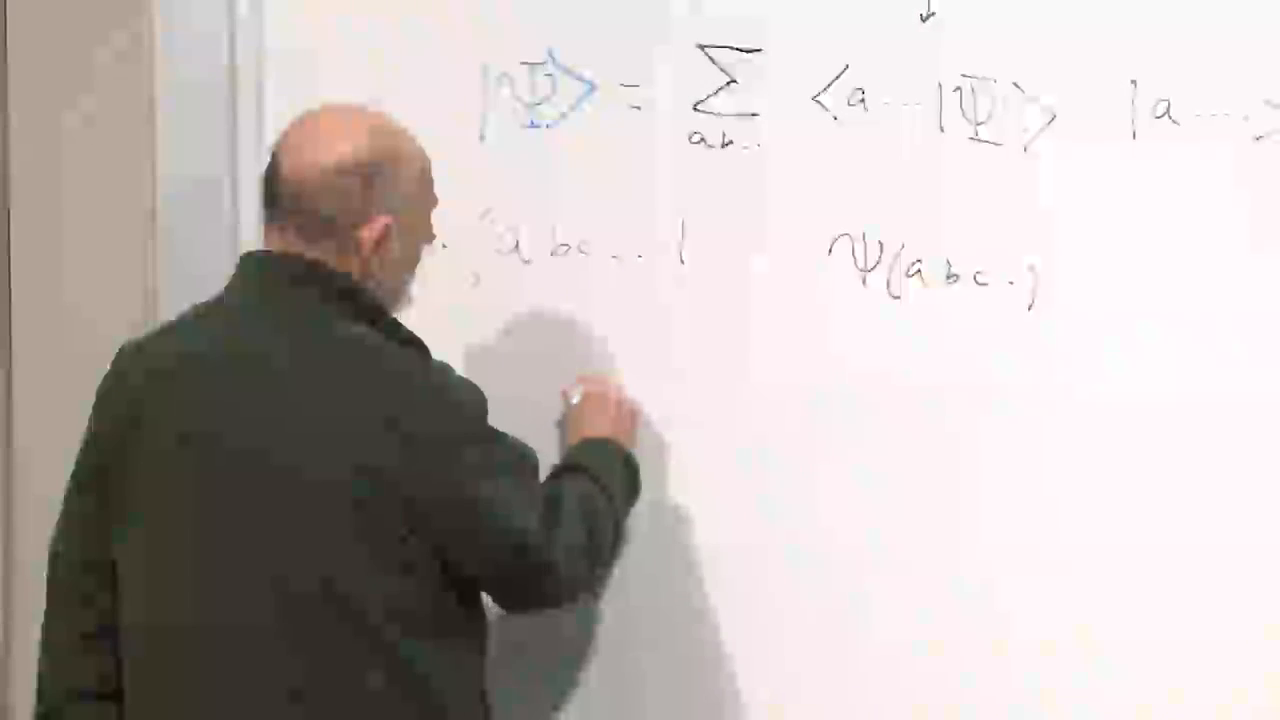
\includegraphics[width=0.88\textwidth]{lecture_07_figure_02.png}
\caption{El valor esperado, escrito como un producto de vectores, desarrollado en coeficientes de la función de onda y elementos de matriz.}
\lectureframe{00:14:08}
\end{figure}

Dividamos ahora el sistema en la parte de Alice y la de Bob. Sea \(a\) una etiqueta de base completa para Alice y \(b\) una para Bob:
\begin{equation}
\ket{\Psi}_{AB}
=\sum_{a,b}\Psi(a,b)\ket{a,b}.
\label{eq:l7-composite-expansion}
\end{equation}
Un observable que pertenece solo a Alice se representa en el espacio compuesto mediante
\begin{equation}
L_A=L\otimes I_B,
\end{equation}
por lo que sus elementos de matriz son
\begin{equation}
\bra{a',b'}L_A\ket{a,b}
=L_{a'a}\delta_{b'b}.
\label{eq:l7-alice-local-matrix}
\end{equation}
Del mismo modo, un observable local de Bob tiene la forma
\begin{equation}
M_B=I_A\otimes M,
\qquad
\bra{a',b'}M_B\ket{a,b}
=\delta_{a'a}M_{b'b}.
\label{eq:l7-bob-local-matrix}
\end{equation}
La identidad en el factor que no se toca expresa matemáticamente que la operación de Alice actúa sobre Alice y la de Bob sobre Bob.

Al sustituir la Ecuación~\eqref{eq:l7-alice-local-matrix} en el valor esperado se obtiene
\begin{equation}
\expect{L_A}
=\sum_{a',a,b}
\Psi^*(a',b)L_{a'a}\Psi(a,b).
\label{eq:l7-local-expectation}
\end{equation}
Esta fórmula ya contiene la matriz de densidad reducida; la reorganizaremos después de ver primero qué implica la factorización.

\begin{classroomqa}
\audiencequestion{¿Por qué queda un solo índice de Bob en la Ecuación~\eqref{eq:l7-local-expectation}?}
\lecturerresponse{La identidad en el espacio de Bob aporta \(\delta_{b'b}\). Igualas las etiquetas del bra y del ket del lado de Bob, y así la suma doble sobre \(b',b\) se reduce a una sola suma sobre \(b\).}
\end{classroomqa}

\begin{classroomqa}
\audiencequestion{¿Necesita Alice saber qué base usa Bob?}
\lecturerresponse{Ninguna predicción física depende de la base de Bob. La suma sobre una base completa de Bob es una resolución de la identidad. Otra base de Bob cambia las componentes individuales \(\Psi(a,b)\), pero no el valor esperado de Alice.}
\end{classroomqa}

\section{Estados producto y correlaciones}

En un estado producto, la función de onda conjunta se factoriza:
\begin{equation}
\Psi(a,b)=\psi_A(a)\phi_B(b).
\label{eq:l7-wavefunction-factorization}
\end{equation}
Sustituyamos esto en la Ecuación~\eqref{eq:l7-local-expectation}:
\begin{align}
\expect{L_A}
&=\sum_{a',a,b}
\psi_A^*(a')\phi_B^*(b)
L_{a'a}
\psi_A(a)\phi_B(b) \\
&=\left[
\sum_{a',a}\psi_A^*(a')L_{a'a}\psi_A(a)
\right]
\left[
\sum_b|\phi_B(b)|^2
\right] \\
&=\bra{\psi_A}L\ket{\psi_A}.
\label{eq:l7-product-local-expectation}
\end{align}
La normalización de Bob hace que su factor valga uno. Por tanto, Alice tiene exactamente las mismas estadísticas locales que habría tenido si nunca se hubiera introducido el sistema de Bob.

\begin{figure}[htbp]
\centering
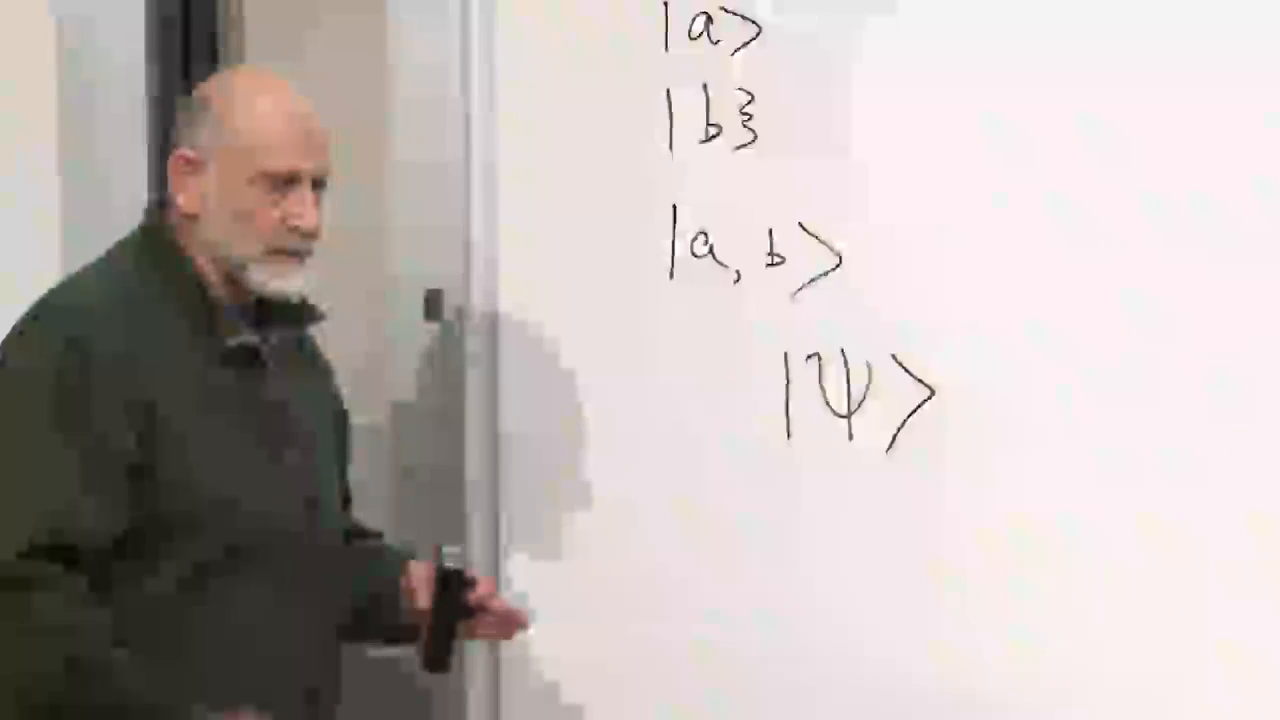
\includegraphics[width=0.88\textwidth]{lecture_07_figure_03.png}
\caption{Factorización de la función de onda conjunta y separación correspondiente de los valores esperados locales.}
\lectureframe{00:29:18}
\end{figure}

El producto de un observable de Alice por uno de Bob tiene elementos de matriz
\begin{equation}
\bra{a',b'}L_A M_B\ket{a,b}
=L_{a'a}M_{b'b}.
\end{equation}
En un estado producto, su valor esperado se separa:
\begin{equation}
\expect{L_A M_B}
=\expect{L_A}\expect{M_B}.
\label{eq:l7-product-correlation-factorization}
\end{equation}
Por tanto, es natural definir la correlación conectada
\begin{equation}
C(L,M)
=\expect{L_A M_B}
-\expect{L_A}\expect{M_B}.
\label{eq:l7-connected-correlation}
\end{equation}
Todo estado producto satisface \(C(L,M)=0\) para cualquier par de observables locales. A la inversa, para un estado bipartito puro, el entrelazamiento garantiza que algún par de observables locales tenga una correlación conectada distinta de cero.

\begin{classroomqa}
\audiencequestion{¿Significa \(L_A M_B\) que primero se mide a Bob y luego a Alice?}
\lecturerresponse{No. Los operadores actúan sobre vectores de estado; los aparatos realizan mediciones. El producto significa que actúa \(M_B\) y luego actúa \(L_A\). Como los operadores ocupan factores tensoriales distintos, \([L_A,M_B]=0\), así que su orden matemático no importa. El protocolo de laboratorio para estimar el valor esperado conjunto es otra cuestión.}
\end{classroomqa}

\begin{classroomqa}
\audiencequestion{¿Puede estar entrelazado el estado aunque una correlación elegida se anule?}
\lecturerresponse{Desde luego. Que \(C(L,M)\) se anule solo indica que este par concreto de observables no está correlacionado. Para establecer la factorización de un estado puro, deben factorizarse todas las correlaciones cruzadas locales. Además, una correlación parcial no implica necesariamente un entrelazamiento parcial en algún sentido sencillo que pueda expresarse con un único número; esa información está contenida en todo el espectro de la matriz de densidad reducida.}
\end{classroomqa}

\begin{classroomqa}
\audiencequestion{¿Todo estado correlacionado está entrelazado?}
\lecturerresponse{Para los estados puros que estamos tratando, las correlaciones que no se factorizan revelan el entrelazamiento. En estados mixtos, las correlaciones clásicas ordinarias también pueden hacer que \(C(L,M)\neq0\). Por tanto, el criterio posterior basado en la matriz de densidad debe matizarse según se sepa o no que el estado del todo es puro.}
\end{classroomqa}

\section{El singlete: un todo definido con partes indefinidas}

Sea \(\boldsymbol{\sigma}\) el operador que actúa sobre el espín de Bob y \(\boldsymbol{\tau}\) el que actúa sobre el de Alice. El estado singlete es
\begin{equation}
\ket{S}
=\frac{1}{\sqrt2}
\left(\ket{u d}-\ket{d u}\right),
\label{eq:l7-singlet}
\end{equation}
donde el primer lugar corresponde a Bob y el segundo a Alice. Ningún espín tiene una componente \(z\) definida:
\begin{equation}
\expect{\sigma_z}=0,
\qquad
\expect{\tau_z}=0.
\label{eq:l7-singlet-local-z}
\end{equation}
Sin embargo, su producto tiene un valor definido:
\begin{equation}
\expect{\sigma_z\tau_z}=-1.
\label{eq:l7-singlet-product-z}
\end{equation}
Toda medición de \(z\) produce resultados opuestos.

La invariancia rotacional hace que la afirmación sea independiente de la dirección. Para cualquier vector unitario \(\mathbf n\),
\begin{equation}
\expect{\boldsymbol{\sigma}\cdot\mathbf n}
=\expect{\boldsymbol{\tau}\cdot\mathbf n}=0,
\qquad
\expect{
(\boldsymbol{\sigma}\cdot\mathbf n)
(\boldsymbol{\tau}\cdot\mathbf n)
}=-1.
\label{eq:l7-singlet-any-axis}
\end{equation}
Más generalmente,
\begin{equation}
\expect{\sigma_i\tau_j}=-\delta_{ij}.
\label{eq:l7-singlet-correlation-tensor}
\end{equation}
Cada parte está completamente despolarizada, mientras que los resultados para componentes en ejes iguales están perfectamente anticorrelacionados.

\begin{figure}[htbp]
\centering
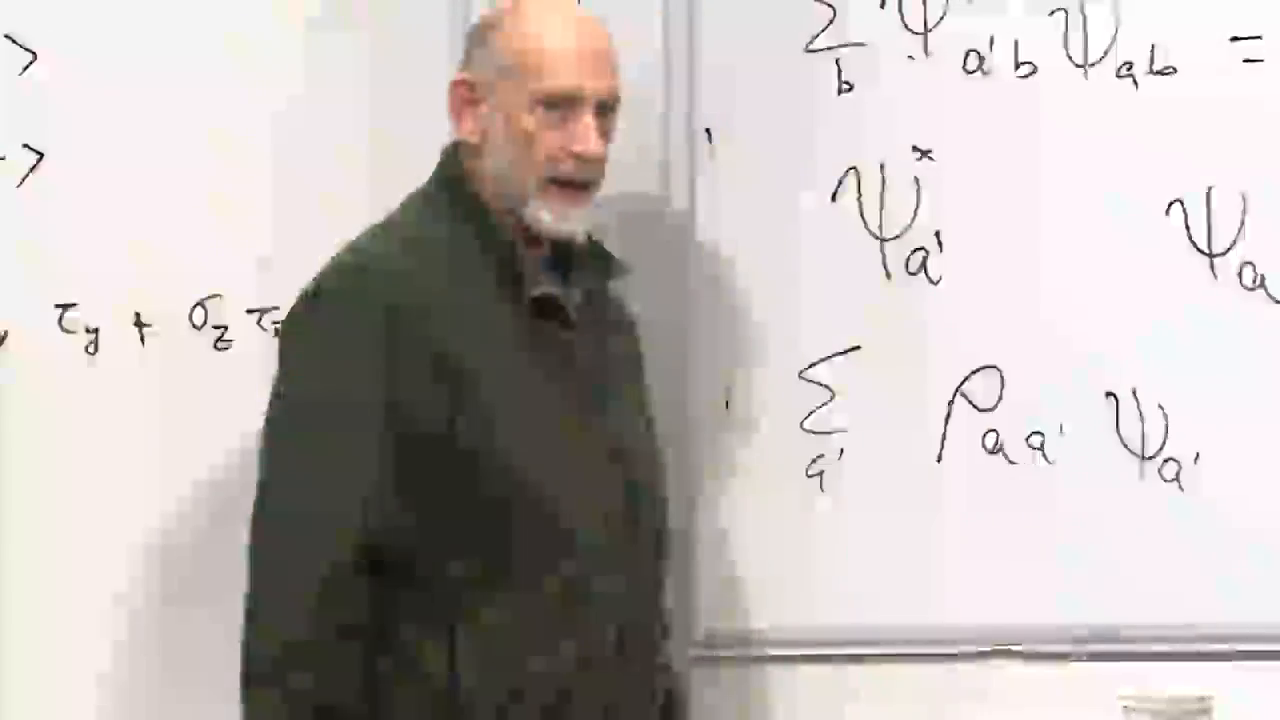
\includegraphics[width=0.88\textwidth]{lecture_07_figure_04.png}
\caption{Para el singlete, el valor medio del espín local de cada parte se anula, mientras que el producto de componentes iguales vale \(-1\).}
\lectureframe{00:38:28}
\end{figure}

Esta es la inversión característica que produce el entrelazamiento. Para un espín aislado en un estado puro, existe alguna dirección en la que su espín está definido. En el singlete, ninguna dirección hace que el espín local de una u otra parte esté definido. Sin embargo, el estado compuesto es puro y está completamente especificado. Sabemos tanto como permite la mecánica cuántica sobre el todo y, aun así, no podemos asignar un estado puro a ninguna de sus partes.

\begin{classroomqa}
\audiencequestion{Si conocemos exactamente el estado del todo, ¿por qué no podemos inferir un estado definido para cada espín?}
\lecturerresponse{Porque el singlete no es un estado producto. Sus coeficientes no se descomponen en una amplitud de Bob multiplicada por una amplitud de Alice. La información reside en las relaciones entre las partes, no en dos funciones de onda locales que existan de forma independiente.}
\end{classroomqa}

\begin{classroomqa}
\audiencequestion{¿Puede ser un operador como \(\sigma_z\) un posible estado del espín?}
\lecturerresponse{No. Un estado es un vector o, más generalmente, un operador de densidad; \(\sigma_z\) es un observable que actúa sobre estados. Un autovector de \(\sigma_z\) es un estado con una componente \(z\) definida, pero el observable y sus autovectores son objetos de distinto tipo.}
\end{classroomqa}

\begin{classroomqa}
\audiencequestion{Cuando escribimos \(\sigma_z\tau_z\ket{S}=-\ket{S}\), ¿hemos realizado una medición?}
\lecturerresponse{No. La ecuación registra cómo actúa un operador sobre un vector. Nos dice que una medición del observable conjunto correspondiente daría con certeza \(-1\), pero el mero hecho de escribir la ecuación de autovalores no implica que se haya incluido ningún detector.}
\end{classroomqa}

\begin{classroomqa}
\audiencequestion{¿Puede un par entrelazado estar correlacionado solo parcialmente?}
\lecturerresponse{Sí. La anticorrelación perfecta es una propiedad especial del singlete para ejes iguales. Otros estados entrelazados pueden tener correlaciones más débiles, e incluso el singlete da \(-\mathbf a\cdot\mathbf b\) en vez de \(-1\) cuando los dos ejes son distintos. El entrelazamiento se refiere a la imposibilidad de factorizar el estado, no a la concordancia o discrepancia perfecta en todas las mediciones elegidas.}
\end{classroomqa}

\section{Preparación del singlete mediante relajación energética}

El operador de dos espines invariante ante rotaciones
\begin{equation}
\boldsymbol{\sigma}\cdot\boldsymbol{\tau}
=\sigma_x\tau_x+\sigma_y\tau_y+\sigma_z\tau_z
\label{eq:l7-spin-dot-spin}
\end{equation}
organiza el espacio de estados de cuatro dimensiones. Para el singlete,
\begin{equation}
(\boldsymbol{\sigma}\cdot\boldsymbol{\tau})\ket{S}
=-3\ket{S},
\label{eq:l7-singlet-dot-eigenvalue}
\end{equation}
mientras que cada uno de los tres estados triplete tiene autovalor \(+1\).

\begin{figure}[htbp]
\centering
\includegraphics[width=0.88\textwidth]{lecture_07_figure_05.png}
\caption{El acoplamiento invariante ante rotaciones \(\boldsymbol{\sigma}\cdot\boldsymbol{\tau}\) y su papel en la separación de los sectores singlete y triplete.}
\lectureframe{00:52:33}
\end{figure}

Supongamos que el hamiltoniano de interacción contiene
\begin{equation}
H_{\mathrm{int}}
=J\,\boldsymbol{\sigma}\cdot\boldsymbol{\tau}.
\label{eq:l7-exchange-hamiltonian}
\end{equation}
Para un acoplamiento antiferromagnético \(J>0\), el singlete está por debajo del triplete en una diferencia de energía de
\begin{equation}
\Delta E=4J.
\end{equation}
Acerque los espines, permita que los componentes de mayor energía decaigan emitiendo un fotón, un fonón u otra excitación, y el par se relajará hacia el singlete. Después, los espines pueden separarse conservando su estado conjunto, siempre que la separación no introduzca rotaciones de espín no controladas ni cierre la brecha de energía con demasiada brusquedad.

La misma lógica energética aparece en sistemas atómicos. En el positronio, por ejemplo, el acoplamiento de los espines del electrón y el positrón separa las configuraciones singlete y triplete. Una diferencia de energía también es una diferencia de masa mediante \(E=mc^2\), aunque la espectroscopia suele expresar el desdoblamiento como energía o frecuencia.

\begin{classroomqa}
\audiencequestion{¿Es siempre el singlete el estado fundamental de dos espines que interactúan?}
\lecturerresponse{No. Es el estado fundamental para el signo \(J>0\) en la Ecuación~\eqref{eq:l7-exchange-hamiltonian}. Al invertir el signo, el triplete queda a menor energía. El argumento de preparación depende de la interacción real y del orden de las energías, no de la mera existencia de dos espines.}
\end{classroomqa}

\begin{classroomqa}
\audiencequestion{¿Se puede medir \(\boldsymbol{\sigma}\cdot\boldsymbol{\tau}\) midiendo por separado las tres componentes?}
\lecturerresponse{No en un mismo par mediante tres mediciones locales simultáneas del espín: \(\sigma_x,\sigma_y,\sigma_z\) son incompatibles, al igual que las tres componentes de \(\tau\). Su valor esperado puede reconstruirse a partir de tres subensambles medidos a lo largo de \(x,y,z\), o el observable singlete--triplete puede medirse directamente con un aparato conjunto adecuado.}
\end{classroomqa}

\begin{classroomqa}
\audiencequestion{Después de separar los espines, ¿deben seguir interactuando para permanecer entrelazados?}
\lecturerresponse{No. La interacción es necesaria para preparar o modificar el estado, pero, una vez preparado el singlete, la evolución unitaria puede conservar su entrelazamiento sin que siga actuando una fuerza entre las partículas. Los campos magnéticos locales pueden rotar los dos factores, pero las rotaciones unitarias locales no destruyen por sí solas el entrelazamiento.}
\end{classroomqa}

\section{La matriz de densidad reducida}

Volvamos al valor esperado local de Alice:
\begin{equation}
\expect{L_A}
=\sum_{a',a,b}
\Psi^*(a',b)L_{a'a}\Psi(a,b).
\end{equation}
Reagrupemos los factores que no pertenecen a \(L\):
\begin{equation}
\expect{L_A}
=\sum_{a',a}
\left[
\sum_b\Psi(a,b)\Psi^*(a',b)
\right]L_{a'a}.
\label{eq:l7-regrouped-expectation}
\end{equation}
La expresión entre corchetes es la matriz de densidad reducida de Alice,
\begin{equation}
(\rho_A)_{aa'}
=\sum_b\Psi(a,b)\Psi^*(a',b).
\label{eq:l7-reduced-density-components}
\end{equation}
En notación independiente de la base,
\begin{equation}
\rho_A
=\operatorname{Tr}_B\ket{\Psi}\bra{\Psi},
\label{eq:l7-partial-trace}
\end{equation}
y todo valor esperado de un observable local de Alice es
\begin{equation}
\expect{L_A}
=\operatorname{Tr}_A(\rho_A L).
\label{eq:l7-density-expectation}
\end{equation}

\begin{figure}[htbp]
\centering
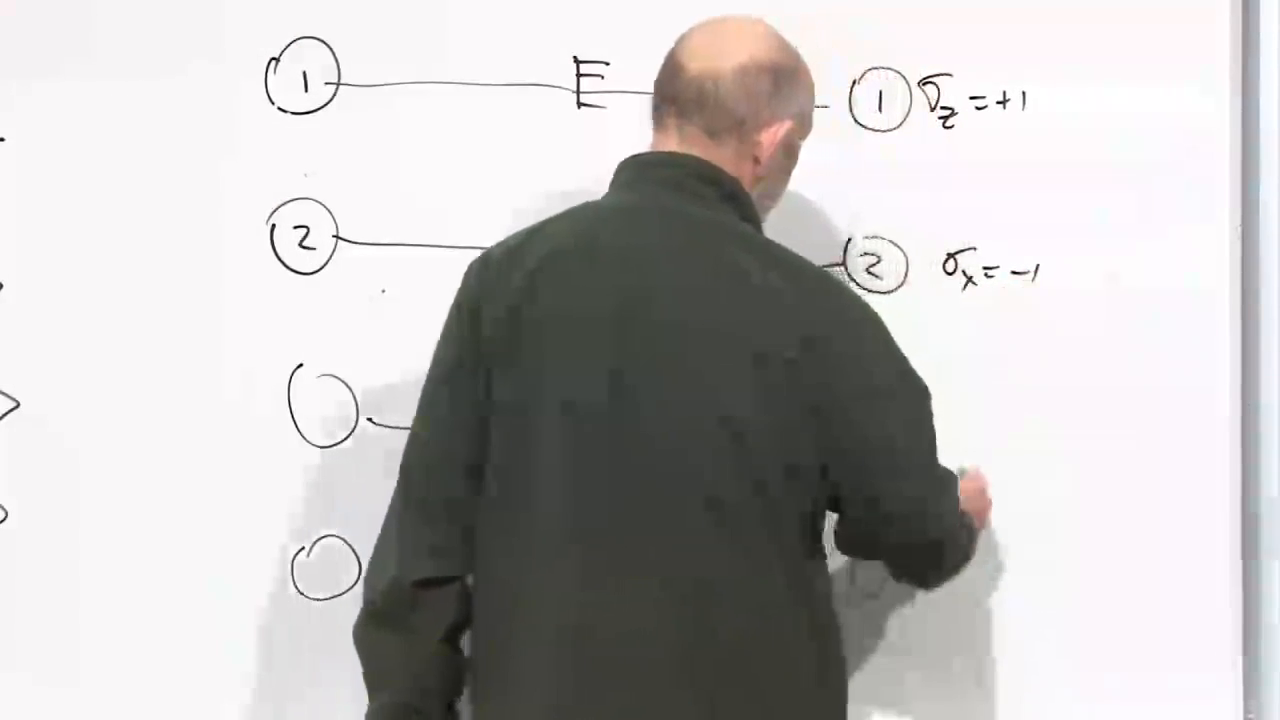
\includegraphics[width=0.88\textwidth]{lecture_07_figure_06.png}
\caption{La matriz de densidad de Alice, obtenida al sumar las amplitudes conjuntas sobre la etiqueta de la base de Bob.}
\lectureframe{01:02:33}
\end{figure}

La matriz de densidad reducida es hermítica, positiva y está normalizada:
\begin{equation}
\rho_A^\dagger=\rho_A,
\qquad
\bra{\chi}\rho_A\ket{\chi}\geq0,
\qquad
\operatorname{Tr}\rho_A=1.
\label{eq:l7-density-properties}
\end{equation}
Contiene exactamente la información necesaria para todas las mediciones restringidas a Alice. Si dos estados globales producen la misma \(\rho_A\), ningún experimento realizado solo por Alice puede distinguirlos.

\begin{classroomqa}
\audiencequestion{¿Mide Alice la matriz de densidad como si fuera un único observable?}
\lecturerresponse{No en una sola medición. La matriz de densidad es el objeto a partir del cual se calculan todas las probabilidades de medición locales. Si dispone de muchos sistemas preparados de forma idéntica, Alice puede reconstruirla mediante tomografía: mide un conjunto suficiente de observables e infiere la matriz a partir de sus valores esperados.}
\end{classroomqa}

\begin{classroomqa}
\audiencequestion{¿Por qué se suma sobre Bob en lugar de seleccionar uno de sus estados?}
\lecturerresponse{Porque Alice no dispone de información sobre los resultados de Bob. La traza parcial suma sobre una base completa de Bob y da el estado local no condicionado. Seleccionar en cambio un resultado de Bob produciría un estado condicionado, una operación distinta que requiere conocer ese resultado.}
\end{classroomqa}

Para un estado producto \(\Psi(a,b)=\psi_A(a)\phi_B(b)\),
\begin{align}
(\rho_A)_{aa'}
&=\sum_b
\psi_A(a)\phi_B(b)
\psi_A^*(a')\phi_B^*(b) \\
&=\psi_A(a)\psi_A^*(a')
\sum_b|\phi_B(b)|^2 \\
&=\psi_A(a)\psi_A^*(a').
\end{align}
Así pues,
\begin{equation}
\rho_A=\ket{\psi_A}\bra{\psi_A}.
\label{eq:l7-pure-projector}
\end{equation}
Esto es un proyector de rango uno. Al actuar sobre \(\ket{\psi_A}\) da
\begin{equation}
\rho_A\ket{\psi_A}
=\ket{\psi_A}\braket{\psi_A}{\psi_A}
=\ket{\psi_A},
\label{eq:l7-density-on-state}
\end{equation}
mientras que, para todo \(\ket{\chi}\) ortogonal a \(\ket{\psi_A}\),
\begin{equation}
\rho_A\ket{\chi}
=\ket{\psi_A}\braket{\psi_A}{\chi}
=0.
\label{eq:l7-density-on-orthogonal}
\end{equation}

\begin{figure}[htbp]
\centering
\includegraphics[width=0.88\textwidth]{lecture_07_figure_07.png}
\caption{Una matriz de densidad de estado producto que actúa como proyector: autovalor \(1\) en la dirección de \(\ket{\psi_A}\) y \(0\) sobre los vectores ortogonales.}
\lectureframe{01:09:43}
\end{figure}

\section{El espectro de la matriz de densidad y el entrelazamiento}

Los autovalores de \(\rho_A\) son no negativos y suman uno. Para un estado puro del todo:
\begin{itemize}
\item un único autovalor no nulo, igual a \(1\), significa que el estado es producto;
\item más de un autovalor no nulo significa que el estado está entrelazado;
\item autovalores iguales en todo el soporte local disponible corresponden a un entrelazamiento máximo.
\end{itemize}
La afirmación se ve con mayor claridad mediante una descomposición de Schmidt,
\begin{equation}
\begin{aligned}
\ket{\Psi}_{AB}
&=\sum_{r=1}^{R}\sqrt{\lambda_r}
\ket{r}_A\ket{r}_B,\\
\lambda_r&\geq0,
\qquad
\sum_r\lambda_r=1.
\end{aligned}
\label{eq:l7-schmidt}
\end{equation}
para la cual
\begin{equation}
\rho_A=\sum_{r=1}^{R}\lambda_r\ket{r}_A\bra{r}.
\label{eq:l7-schmidt-density}
\end{equation}
El rango de Schmidt \(R\) es uno para un estado producto y mayor que uno para un estado puro entrelazado.

Para el singlete,
\begin{equation}
\rho_A
=\operatorname{Tr}_B\ket{S}\bra{S}
=\frac12\ket{u}\bra{u}
+\frac12\ket{d}\bra{d}
=\frac12 I.
\label{eq:l7-singlet-reduced-density}
\end{equation}
Sus autovalores son
\begin{equation}
\operatorname{spec}(\rho_A)
=\left\{\frac12,\frac12\right\}.
\end{equation}
El estado local de Alice es máximamente mezclado, aunque el estado del par sea puro.

El espectro sugiere una medida cuantitativa. La entropía de von Neumann
\begin{equation}
S(\rho_A)
=-\operatorname{Tr}(\rho_A\log\rho_A)
=-\sum_r\lambda_r\log\lambda_r
\label{eq:l7-entanglement-entropy}
\end{equation}
se anula para un estado puro producto y alcanza \(\log d_A\) para un estado máximamente entrelazado cuando \(d_A\leq d_B\). Podemos dejar para más adelante el uso detallado de la entropía; el espectro ya ofrece la distinción esencial.

\begin{classroomqa}
\audiencequestion{¿Deben ser no nulos todos los autovalores de una matriz de densidad reducida de un estado entrelazado?}
\lecturerresponse{No. Basta con que haya más de un autovalor no nulo. Si el espacio de Alice es grande, un estado entrelazado puede ocupar solo un subespacio de Schmidt de menor dimensión y dejar autovalores adicionales iguales a cero. El entrelazamiento máximo significa que los autovalores son iguales en todo el subsistema más pequeño, no solo entre un subconjunto elegido arbitrariamente.}
\end{classroomqa}

\begin{classroomqa}
\audiencequestion{¿Una matriz de densidad reducida mixta demuestra por sí sola que Alice está entrelazada con Bob?}
\lecturerresponse{Solo si se sabe que el estado global es puro. Un estado local mixto también puede surgir de una mezcla clásica ordinaria en un estado global mixto. Sin embargo, para un estado bipartito puro, la mezcla local equivale exactamente al entrelazamiento entre las dos partes.}
\end{classroomqa}

\begin{classroomqa}
\audiencequestion{¿Pueden todos los momentos de los observables de Alice determinar sus distribuciones de probabilidad?}
\lecturerresponse{En un sistema de dimensión finita, los valores esperados de una base de operadores determinan \(\rho_A\), y \(\rho_A\) determina todas las distribuciones de resultados locales mediante la regla de Born. La reconstrucción requiere un conjunto de copias preparadas de forma idéntica; un único suceso aislado no puede revelar una matriz de densidad.}
\end{classroomqa}

\section{La medición como interacción que entrelaza}

Sustituyamos a Alice y Bob por un espín y un aparato de medición. Sea el aparato un estado listo \(\ket{0}_D\) y un estado activado \(\ket{1}_D\). Una interacción ideal que registra si el espín está hacia arriba puede representarse mediante
\begin{align}
\ket{u}\ket{0}_D&\longrightarrow\ket{u}\ket{1}_D,\\
\ket{d}\ket{0}_D&\longrightarrow\ket{d}\ket{0}_D.
\label{eq:l7-measurement-basis-map}
\end{align}
El detector debe comenzar en un estado listo conocido; de lo contrario, su estado final no proporcionaría un registro inequívoco.

La linealidad determina la evolución de una superposición:
\begin{equation}
\left(\alpha\ket{u}+\beta\ket{d}\right)\ket{0}_D
\longrightarrow
\alpha\ket{u}\ket{1}_D
+\beta\ket{d}\ket{0}_D.
\label{eq:l7-measurement-entanglement}
\end{equation}
A menos que uno de los coeficientes se anule, el estado final está entrelazado. El aparato ha adquirido información precisamente porque su estado del puntero está correlacionado con el espín.

\begin{figure}[htbp]
\centering
\includegraphics[width=0.88\textwidth]{lecture_07_figure_08.png}
\caption{Una medición ideal correlaciona las alternativas de espín con estados distintos del puntero y, de ese modo, crea entrelazamiento.}
\lectureframe{01:20:20}
\end{figure}

Si se conserva solo el espín y se ignora el detector, su estado reducido es
\begin{equation}
\rho_{\mathrm{spin}}
=|\alpha|^2\ket{u}\bra{u}
+|\beta|^2\ket{d}\bra{d},
\label{eq:l7-postmeasurement-reduced-state}
\end{equation}
suponiendo que los registros del puntero sean ortogonales. Los términos de interferencia han desaparecido de la descripción local porque están almacenados en las correlaciones con el aparato.

Ahora hay dos descripciones complementarias. Si se lee el resultado del detector y se condiciona el estado al registro, se asigna al espín la rama correspondiente: \(\ket{u}\) tras una activación o \(\ket{d}\) si no hay activación. Esta es la descripción de colapso. Si se tratan el detector y el espín como un único sistema cerrado, la Ecuación~\eqref{eq:l7-measurement-entanglement} describe una evolución unitaria ordinaria y no se ha eliminado ninguna rama del estado conjunto.

\begin{classroomqa}
\audiencequestion{¿La medición es algo que va más allá del entrelazamiento?}
\lecturerresponse{En el nivel de la dinámica sistema--aparato, la medición es una interacción que establece una correlación fiable. El colapso es la descripción condicionada que se usa después de seleccionar un registro definido. Considerar esa actualización como fundamental o como relativa al corte elegido es una cuestión interpretativa; las predicciones operativas coinciden.}
\end{classroomqa}

\begin{classroomqa}
\audiencequestion{¿Por qué una medición ideal deja inalterado el autoestado del espín?}
\lecturerresponse{Ese es el requisito de repetibilidad de este modelo. Si la entrada ya es un autoestado del observable medido, el aparato debe registrar su valor sin cambiarlo. Las mediciones reales pueden ser destructivas, pero en ese caso su interacción debe modelarse de otra manera.}
\end{classroomqa}

\section{La jerarquía de observadores}

Una vez que se admite el aparato como sistema cuántico, no hay ninguna razón natural para detenerse ahí. La luz del puntero interactúa con un ojo; las señales del ojo se correlacionan con un cerebro; un observador puede ser observado por otro. El gato de Schr\"odinger y el amigo de Wigner dramatizan la misma estructura anidada:
\begin{equation}
\begin{gathered}
\text{spin}
\longrightarrow
\text{apparatus}
\longrightarrow
\text{cat}\\
\longrightarrow
\text{Schr\"odinger}
\longrightarrow
\text{Wigner}.
\end{gathered}
\label{eq:l7-observer-chain}
\end{equation}
Dentro de cualquier frontera elegida, la cadena puede describirse mediante evolución unitaria y entrelazamiento creciente. Fuera de esa frontera, se emplea el lenguaje de resultados condicionados por el resultado de la medición.

La condición crucial de consistencia es que la frontera pueda desplazarse. Si el gato registra que el espín está hacia arriba, Schr\"odinger debe registrar después un gato que vio el espín hacia arriba, y Wigner debe registrar Schr\"odinger que ese mismo gato registró esa misma historia. La mecánica cuántica no identifica una línea nítida única en la que deba declararse que ocurrió un suceso objetivo. Los gatos, los ojos y los cerebros están hechos de grados de libertad físicos; eximir a uno de ellos de la mecánica cuántica exigiría una ley adicional.

La actitud de Feynman ante la incomodidad resultante era pragmática. El problema conceptual puede ser tan grande que incluso resulte difícil decir si existe, mientras las reglas de cálculo siguen prediciendo todos los experimentos a los que se aplican. El formalismo no pretende imponer una interpretación, sino precisar el origen de la incomodidad: el conocimiento completo de un todo puede coexistir con la ausencia de una descripción de sus partes mediante estados puros.

\begin{classroomqa}
\audiencequestion{Si soy el gato, ¿tengo que trazar la frontera en mí mismo?}
\lecturerresponse{Puedes usar una descripción de colapso para el registro definido que está a tu disposición. Otro observador que te incluya en un sistema aislado mayor puede usar una descripción de estado entrelazado. No se exige que todos tracen la misma frontera, sino que todas las descripciones den registros coherentes cuando los observadores comparen sus resultados más adelante.}
\end{classroomqa}

\begin{classroomqa}
\audiencequestion{¿Dónde ocurre el suceso objetivo: en el átomo, el gato, Schr\"odinger o Wigner?}
\lecturerresponse{El formalismo unitario no selecciona ninguno de esos lugares como frontera privilegiada. Quizá se esté llevando el uso de palabras corrientes como \emph{ocurrir} más allá del contexto en que tienen un significado preciso. Las herramientas formales nos dicen cómo se propagan las correlaciones y qué puede predecir cada observador; decidir cómo interpretar la frontera final es una tarea aparte.}
\end{classroomqa}

\subsection{Acoplamiento débil y lectura imperfecta}

La correspondencia ideal de la Ecuación~\eqref{eq:l7-measurement-basis-map} produce registros perfectamente distinguibles. Una interacción más débil puede dejar los estados del aparato solo parcialmente distinguibles:
\begin{equation}
\alpha\ket{u}\ket{D_u}
+\beta\ket{d}\ket{D_d},
\qquad
0<|\braket{D_d}{D_u}|<1.
\label{eq:l7-weak-measurement}
\end{equation}
En ese caso, el aparato recibe solo información parcial y el entrelazamiento es incompleto. Este es el escenario de una medición débil o no nítida.

Esta situación debe distinguirse de una lectura posterior defectuosa. El detector puede haberse correlacionado por completo con el espín mientras el ojo, el cable, el amplificador o el cerebro no transmiten el registro de manera clara. En el primer caso, la interacción sistema--detector es débil; en el segundo, el detector contiene un buen registro, pero la transferencia posterior de información es ineficiente. La eficiencia del detector puede involucrar cualquiera de las dos etapas, así que hay que identificar el acoplamiento físico antes de atribuir la causa.

\begin{classroomqa}
\audiencequestion{Si la mala visión hace que no se sepa con certeza qué indica el puntero, ¿fue débil la medición cuántica?}
\lecturerresponse{No necesariamente. El espín pudo haber estado fuertemente correlacionado con el aparato, de manera completa, mientras que el canal entre el aparato y el ojo, o entre el ojo y el cerebro, era deficiente. Una medición genuinamente débil significa que el acoplamiento inicial entre el sistema y el--aparato produjo registros que solo eran parcialmente distinguibles.}
\end{classroomqa}

\section{Localidad y ausencia de señalización}

La expresión \emph{acción a distancia} debe recibir un significado operacional. En la física ordinaria, una acción a distancia cambia lo que se puede observar aquí. Si el Sol desapareciera y el movimiento de la Tierra cambiara de inmediato, en vez de hacerlo tras el tiempo que tarda la luz en llegar, se podría usar ese cambio para transmitir información más rápido que la luz. Eso sería una señalización no local genuina.

El entrelazamiento no permite esa señalización. Sea que Bob realice una operación cuántica local representada por los operadores de Kraus \(K_\mu\), con
\begin{equation}
\sum_\mu K_\mu^\dagger K_\mu=I_B.
\end{equation}
Si Alice no llega a conocer el resultado de Bob, el estado conjunto final es
\begin{equation}
\rho'_{AB}
=\sum_\mu
(I_A\otimes K_\mu)\rho_{AB}
(I_A\otimes K_\mu^\dagger).
\end{equation}
Al tomar la traza parcial sobre Bob se obtiene
\begin{equation}
\rho'_A
=\operatorname{Tr}_B\rho'_{AB}
=\operatorname{Tr}_B\rho_{AB}
=\rho_A.
\label{eq:l7-no-signaling}
\end{equation}
Por lo tanto, las probabilidades locales no condicionadas de Alice no cambian según la operación local de Bob que preserve la traza.

Los estados condicionados son distintos. Si Bob mide y obtiene el resultado \(\mu\), Alice puede asignar
\begin{equation}
\rho_{A|\mu}
=\frac{
\operatorname{Tr}_B\!\left[
(I_A\otimes K_\mu)\rho_{AB}
(I_A\otimes K_\mu^\dagger)
\right]
}{p_\mu}.
\label{eq:l7-conditioned-state}
\end{equation}
Pero Alice no puede saber cuál estado \(\rho_{A|\mu}\) corresponde hasta que Bob le comunique \(\mu\) mediante una señal ordinaria. Antes de que llegue el mensaje, debe promediar sobre los resultados:
\begin{equation}
\sum_\mu p_\mu\rho_{A|\mu}=\rho_A.
\label{eq:l7-conditioned-average}
\end{equation}

\begin{classroomqa}
\audiencequestion{¿Cuándo cambia la matriz de densidad de Alice si Bob mide primero?}
\lecturerresponse{Su matriz de densidad no condicionada no cambia. Cuando recibe el resultado de Bob, puede sustituirla por la matriz de densidad condicional correspondiente. Esa actualización refleja información que acaba de estar disponible y no puede utilizarse antes de que llegue el mensaje clásico.}
\end{classroomqa}

\begin{classroomqa}
\audiencequestion{¿La medición de Bob colapsa físicamente el estado de Alice en el mismo instante?}
\lecturerresponse{Las distintas interpretaciones describen de manera diferente la actualización condicional, pero todas concuerdan en lo que se puede comprobar: las probabilidades de los resultados locales de Alice no cambian hasta que dispone de la información de Bob. No se produce ninguna señal controlable instantánea.}
\end{classroomqa}

Imaginemos muchos pares singlete distribuidos en filas numeradas. En un miembro del par, Bob mide \(z\); en otro, \(x\); en otro, \(y\), y así sucesivamente. Los resultados locales de Alice siguen formando una secuencia no sesgada en cada fila:
\begin{equation}
P_A(+|\mathbf a)=P_A(-|\mathbf a)=\frac12.
\label{eq:l7-alice-marginal}
\end{equation}
Nada en su cuaderno revela qué ejes eligió Bob ni qué resultados obtuvo.

\begin{figure}[htbp]
\centering
\includegraphics[width=0.88\textwidth]{lecture_07_figure_09.png}
\caption{Muchos pares preparados independientemente permiten asignar distintos ejes de medición a distintas filas; las estadísticas marginales de Alice no cambian.}
\lectureframe{01:49:00}
\end{figure}

Cuando llega un telegrama, limitado por la velocidad de la luz, que enumera el eje y el resultado de Bob para cada fila, Alice puede ordenar sus registros. Entonces, las mediciones del singlete con el mismo eje darán resultados opuestos para cada par. El mensaje revela correlaciones que ya estaban presentes en las estadísticas conjuntas; no altera retroactivamente la distribución local de frecuencias anterior de Alice.

\begin{classroomqa}
\audiencequestion{¿Podría Alice deducir la elección de Bob a partir de suficientes momentos de sus propios datos?}
\lecturerresponse{Todos los momentos locales de Alice están determinados por \(\rho_A\), y la ecuación~\eqref{eq:l7-no-signaling} deja esa matriz sin cambios. Más copias mejoran su estimación de la misma matriz de densidad local; no revelan la base de Bob ni su resultado.}
\end{classroomqa}

\begin{classroomqa}
\audiencequestion{¿Y si Bob elige un eje distinto para cada miembro del conjunto?}
\lecturerresponse{Alice sigue observando la misma distribución local. Cuando Bob envía la configuración y el resultado de cada fila, ambos pueden comparar las correlaciones condicionales para cada par de ejes. La dependencia respecto de la configuración aparece en las estadísticas conjuntas, no en las estadísticas marginales de Alice.}
\end{classroomqa}

\section{La pregunta de Bell como juego de simulación}

La diferencia entre la ausencia de señalización y la no localidad de Bell se entiende mejor como un problema de simulación clásica. Empecemos con un espín,
\begin{equation}
\ket{\psi}=\alpha_u\ket{u}+\alpha_d\ket{d},
\qquad
|\alpha_u|^2+|\alpha_d|^2=1.
\end{equation}
Un programa clásico puede almacenar las dos amplitudes complejas, hacerlas evolucionar con la ecuación de Schr\"odinger y aceptar una dirección de medición elegida por el usuario. Cuando se ejecuta el comando de medir, el programa calcula las probabilidades de Born, usa un generador de números seudoaleatorios para seleccionar un resultado, lo muestra y actualiza el estado almacenado al estado propio correspondiente. Repetir el proceso reproduce las estadísticas de un espín.

Por tanto, la aleatoriedad por sí sola no marca la diferencia entre la mecánica clásica y la cuántica. Los computadores clásicos pueden generar secuencias que, desde el punto de vista operacional, son suficientemente aleatorias para una simulación, aunque sus algoritmos seudoaleatorios sean deterministas en el fondo.

Para dos espines en un estado producto, también bastan dos computadores separados. El computador de Alice almacena y hace evolucionar \(\ket{\psi_A}\); el de Bob almacena y hace evolucionar \(\ket{\phi_B}\). Cada uno responde solo a su configuración local. Como las probabilidades conjuntas se factoran, no hace falta comunicarse una vez separados los computadores.

Un par entrelazado cambia el problema. Antes del experimento, se pueden juntar las dos máquinas, cargar datos ocultos correlacionados, sincronizar sus relojes e incluso darles semillas aleatorias idénticas. Sin embargo, una vez separadas, cada salida debe depender solo de la configuración de medición local y de la información compartida proporcionada de antemano. El teorema de Bell demuestra que ningún esquema local de variables ocultas de ese tipo reproduce todas las correlaciones cuánticas para configuraciones elegidas libremente.

\begin{figure}[htbp]
\centering
\includegraphics[width=0.88\textwidth]{lecture_07_figure_10.png}
\caption{El modelo de computadores separados: los programas locales pueden compartir datos de preparación, pero, una vez separados, no pueden comunicarse las configuraciones de medición.}
\lectureframe{02:00:00}
\end{figure}

Si quedan cables entre los computadores para intercambiar configuraciones y resultados, la simulación puede reproducir las correlaciones. Pero entonces el par ya no constituye un modelo local genuinamente separado: funciona como un único computador conectado. El obstáculo no es la computación clásica en abstracto. Una sola máquina clásica global puede simular sistemas cuánticos finitos almacenando la función de onda conjunta completa, aunque la memoria requerida por lo general crece exponencialmente con el número de subsistemas. El obstáculo de Bell concierne a la descomposición en máquinas locales que operan de manera independiente.

\begin{classroomqa}
\audiencequestion{¿Por qué no pueden usar sencillamente los dos computadores la misma secuencia de números aleatorios?}
\lecturerresponse{La aleatoriedad compartida ya está permitida en un modelo local de variables ocultas. Puede predeterminar respuestas correlacionadas, pero cada respuesta debe servir para cualquier configuración de medición que pudiera elegirse después en ese lado. Las desigualdades de Bell expresan las restricciones que cumplen todas esas estrategias locales preestablecidas; las correlaciones cuánticas violan esas restricciones.}
\end{classroomqa}

\begin{classroomqa}
\audiencequestion{¿Tienen que depender los números aleatorios de las direcciones de medición?}
\lecturerresponse{Una salida local puede depender de su propia dirección local y de los datos ocultos compartidos, pero no de la dirección distante elegida después de la separación. Permitir que dependa de ambas configuraciones requiere comunicación, retrocausalidad o el abandono del supuesto habitual de independencia de la medición. El teorema de Bell hace explícitos estos supuestos, en lugar de ocultarlos bajo la palabra \emph{aleatorio}.}
\end{classroomqa}

\begin{classroomqa}
\audiencequestion{¿Tendrían éxito dos computadores cuánticos separados donde fracasan los programas clásicos?}
\lecturerresponse{Pueden tener éxito si comparten grados de libertad cuánticos entrelazados. En ese caso, los computadores no simulan el entrelazamiento mediante registros clásicos locales: lo poseen físicamente. Sus resultados locales siguen sin poder transmitir un mensaje controlable más rápido que la luz.}
\end{classroomqa}

\begin{classroomqa}
\audiencequestion{¿Puede un computador clásico ordinario simular el par entero?}
\lecturerresponse{Sí. Puede almacenar las cuatro amplitudes conjuntas y calcular en un solo lugar todas las probabilidades de medición. Para muchas partículas, esta simulación directa se vuelve costosa porque la dimensión del espacio de Hilbert crece exponencialmente, pero no hay contradicción con Bell cuando toda la información está disponible globalmente dentro de una misma máquina.}
\end{classroomqa}

\begin{classroomqa}
\audiencequestion{¿Demuestra entonces el teorema de Bell que existe una acción a distancia ordinaria?}
\lecturerresponse{Demuestra que las explicaciones locales de variables ocultas que satisfacen los supuestos de Bell no pueden reproducir las correlaciones observadas. No proporciona a Alice ni a Bob un canal de señalización superlumínico. La no localidad de Bell y la comunicación operacional más rápida que la luz son afirmaciones distintas.}
\end{classroomqa}

\section{¿Qué se puede aprender localmente?}

No deben confundirse los observables locales con los conjuntos. Bob puede medir \(\sigma_x\) y Alice puede medir \(\tau_x\); más tarde, al comparar sus registros, estiman
\begin{equation}
\expect{\sigma_x\tau_x}.
\end{equation}
Ninguno de los aparatos locales mide por sí solo ese producto. El escalar rotacional
\begin{equation}
\boldsymbol{\sigma}\cdot\boldsymbol{\tau}
=\sigma_x\tau_x+\sigma_y\tau_y+\sigma_z\tau_z
\end{equation}
requiere usar distintos subconjuntos para los tres términos o un nuevo aparato conjunto que distinga los sectores singlete y triplete. Con los medidores de espín locales originales no se pueden obtener los productos de las tres componentes incompatibles para un mismo par.

\begin{classroomqa}
\audiencequestion{¿Hay observables del sistema completo que los aparatos originales de Alice y Bob no puedan medir por separado?}
\lecturerresponse{Sí. Se puede estimar un producto único como \(\sigma_x\tau_x\) mediante dos mediciones locales del componente \(x\), seguidas de una comparación. La suma \(\boldsymbol{\sigma}\cdot\boldsymbol{\tau}\) no se puede formar a partir de lecturas simultáneas de \(x,y,z\) en un mismo par. Hace falta una medición genuinamente conjunta de los sectores singlete--triplete o conjuntos separados para los términos incompatibles.}
\end{classroomqa}

Bob no puede inferir el entrelazamiento a partir de un solo evento. Sin embargo, con muchas copias preparadas de manera idéntica, puede reconstruir su matriz de densidad reducida. Para un cúbit,
\begin{equation}
\rho_B
=\frac12\left(
I+\mathbf r\cdot\boldsymbol{\sigma}
\right),
\label{eq:l7-bloch-density}
\end{equation}
y las mediciones a lo largo de varios ejes determinan el vector de Bloch \(\mathbf r\). Si \(|\mathbf r|=1\), el estado local de Bob es puro; si \(|\mathbf r|<1\), es mixto. En el caso especial en que se sabe que la preparación global es el mismo estado puro en todos los ensayos, que el estado local sea mixto demuestra que Bob está entrelazado con algo fuera de su subsistema.

Para un producto de dos espines puros, Bob puede buscar la dirección de polarización \(\mathbf n=\mathbf r/|\mathbf r|\). A lo largo de ese eje, las mediciones repetidas dan siempre una respuesta definida. Para el singlete, \(\mathbf r=0\), por lo que todos los ejes siguen siendo aleatorios localmente. La búsqueda nunca encuentra una dirección de polarización.

\begin{classroomqa}
\audiencequestion{¿Puede Bob descubrir el entrelazamiento sin hablar con Alice?}
\lecturerresponse{A partir de un conjunto, puede descubrir que su propio estado reducido es mixto. Si además sabe que cada par se preparó en el mismo estado puro global, puede inferir que hay entrelazamiento a través de la frontera. Sin ese supuesto de pureza, su estado mixto también podría deberse a una mezcla de preparaciones clásicas, y los datos locales por sí solos no permitirían decidir entre ambas posibilidades.}
\end{classroomqa}

\begin{classroomqa}
\audiencequestion{¿Por qué hacen falta muchos sistemas preparados de manera idéntica?}
\lecturerresponse{Cada medición de espín produce un solo resultado y, por lo general, perturba esa copia. Por eso, la tomografía distribuye las mediciones incompatibles entre un conjunto preparado mediante el mismo procedimiento. La matriz de densidad y su espectro son propiedades estadísticas que se infieren de esos ensayos repetidos, no etiquetas que revele una sola partícula.}
\end{classroomqa}

La lógica vuelve ahora al punto de partida. El entrelazamiento no es una vaga idea de compartir un estado. Consiste en que un estado conjunto puro no se factoriza, algo que se manifiesta localmente en una matriz de densidad reducida que no es un proyector y, en conjunto, en correlaciones que no pueden reproducirse mediante una contabilidad clásica en sistemas separados. El todo puede conocerse perfectamente mientras cada parte permanece en un estado mixto. Este hecho hace posible la medición, preserva la ausencia de señalización y proporciona la estructura que pondrá a prueba el teorema de Bell.
